% Asset ID: FA21InequalitiesTikZ-003
% Source: FP1 PDF Ex 4B + teacher transcript
% Related lesson section: Section 9; Worked Example 6
% Purpose: Graphical inequality sketch for 7x/(3x+1)<4-x.
% Boundary status: Internal portal enrichment, not official CCEA Further Mathematics specification content.
\documentclass[tikz,border=8pt]{standalone}
\usepackage{amsmath}
\usepackage{xcolor}
\definecolor{Canvas}{HTML}{FAF9F6}
\definecolor{Ink}{HTML}{2C2C2E}
\definecolor{LineSoft}{HTML}{E5E5EA}
\definecolor{Gold}{HTML}{C5A059}
\definecolor{WarmPink}{HTML}{FBEFEF}
\begin{document}

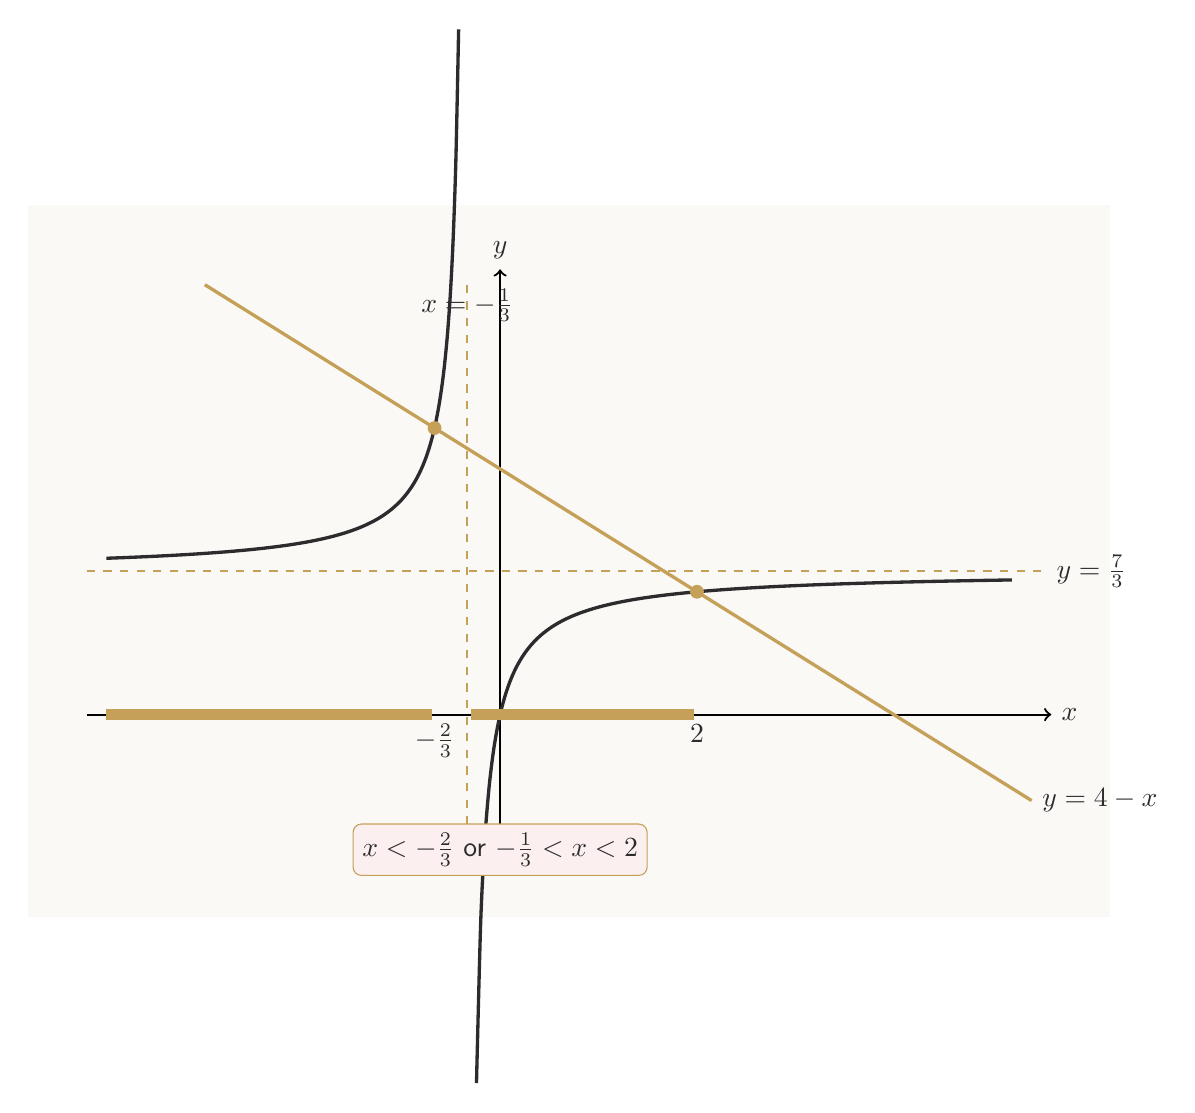
\begin{tikzpicture}[x=1.25cm,y=0.78cm,every node/.style={font=\sffamily,text=Ink}]
\fill[Canvas] (-4.8,-3.3) rectangle (6.2,8.3);
\draw[->,thick] (-4.2,0)--(5.6,0) node[right] {$x$};
\draw[->,thick] (0,-2.6)--(0,7.25) node[above] {$y$};
\draw[Gold,dashed,thick] (-0.333,-2.6)--(-0.333,7.1) node[below] {$x=-\frac13$};
\draw[Gold,dashed,thick] (-4.2,2.333)--(5.55,2.333) node[right] {$y=\frac73$};
\draw[Ink,very thick,domain=-4:-0.42,samples=130,smooth] plot (\x,{7*\x/(3*\x+1)});
\draw[Ink,very thick,domain=-0.24:5.2,samples=130,smooth] plot (\x,{7*\x/(3*\x+1)});
\draw[Gold,very thick] (-3,7)--(5.4,-1.4) node[right] {$y=4-x$};
\fill[Gold] (-0.666,4.666) circle (2.5pt);\fill[Gold] (2,2) circle (2.5pt);
\draw[Gold,line width=4pt] (-4,0)--(-0.69,0);\draw[Gold,line width=4pt] (-0.30,0)--(1.97,0);
\node[below] at (-0.666,0) {$-\frac23$};\node[below] at (2,0) {$2$};
\node[fill=WarmPink,draw=Gold,rounded corners=3pt] at (0,-2.2) {$x<-\frac23$ or $-\frac13<x<2$};
\end{tikzpicture}

\end{document}
